%%----------------------------------------------------------------------------
%% Onderzoekstechnieken: Analyse van 1 variabele
%%----------------------------------------------------------------------------

\documentclass[aspectratio=169]{beamer}

%==============================================================================
% Aanloop
%==============================================================================

%---------- Vormgeving --------------------------------------------------------

\usetheme{hogent}

\usecolortheme{hgwhite} % witte achtergrond, zwarte tekst

\usepackage{graphicx,multicol}
\usepackage{comment,enumerate,hyperref}
\usepackage{amsmath,amsfonts,amssymb}
\usepackage[dutch]{babel}
\usepackage{multirow}
\usepackage{eurosym}
\usepackage{listings}
\usepackage{textcomp}
\usepackage{framed}
\usepackage{wrapfig}
\usepackage{tabu} %needed for \tabulinesep
\usepackage{wrapfig}
\usepackage{pgf-pie}
\usepackage{pgfplots}
\usepackage{booktabs}

%---------- Configuratie ------------------------------------------------------

\pgfplotsset{compat=1.16}
\usetikzlibrary{arrows,shapes,backgrounds,positioning,shadows}
\usetikzlibrary{pgfplots.statistics}

%---------- Commando-definities -----------------------------------------------

\newcommand{\tabitem}{~~\llap{\textbullet}~~}
\newcommand{\alertbox}[2][hgblue]{%
  \setbeamercolor{alertbox}{bg=#1,fg=white}
  \begin{beamercolorbox}[sep=2pt,center]{alertbox}
    \textbf{#2}
  \end{beamercolorbox}
}

%---------- Info over de presentatie ------------------------------------------

\title{Chapter 3. Univariate Analysis}
\subtitle{Research techniques}
\author{Jens Buysse \and Wim {De Bruyn} \and Pieter-Jan Maenhaut \and Bert {Van Vreckem}}
\date{AY 2019-2020}

%==============================================================================
% Inhoud presentatie
%==============================================================================

\begin{document}

\begin{frame}
  \maketitle
\end{frame}

\begin{frame}
  \frametitle{What's on the menu?}
  
  \tableofcontents
\end{frame}

\begin{frame}
  \frametitle{Learning Goals}
  
  \begin{itemize}
    \item Descriptive statistics
    \item Central tendency and dispersion for each measurement level
    \item Know formulas, being able to calculate
    \item Suitable visualization techniques for each measurement level
  \end{itemize}
\end{frame}

\section{Central Tendency and Dispersion}

\begin{frame}
  \frametitle{How tall are my friends?}
  
  Remember our superheroes:
  
  \begin{tikzpicture}[xscale=4,yscale=2]
  \draw (0,2) -- (0,0);
  \foreach \num/\label in {0/0, 0.2/20, .4/40, .6/60, .8/80, 1/100, 1.2/120, 1.4/140, 1.6/160, 1.8/180, 2/200}{%
    \draw (0, \num) -- (2.5, \num);
    \draw[shift={(0, \num)}] (1pt,0pt) -- (-1pt,0pt) node[left] {\scriptsize \label};
  }
  
  \node[anchor=north] (hero1) at (0.3,1.5)
  {\includegraphics[height=2.9cm]{les2-hero-1}};
  \node[anchor=north] (hero2) at (0.8,2.05)
  {\includegraphics[height=4cm]{les2-hero-2}};
  \node[anchor=north] (hero3) at (1.3,1.575)
  {\includegraphics[height=3.1cm]{les2-hero-3}};
  \node[anchor=north] (hero4) at (1.8,2.1)
  {\includegraphics[height=4.1cm]{les2-hero-4}};
  \node[anchor=north] (hero5) at (2.3,1.95)
  {\includegraphics[height=3.8cm]{les2-hero-5}};
  
  \node (size1) at (0.3, 1.5) {\scriptsize 141 cm};
  \node (size2) at (0.8, 2.1) {\scriptsize 198 cm};
  \node (size3) at (1.3, 1.51) {\scriptsize 143 cm};
  \node (size4) at (1.8, 2.15) {\scriptsize 201 cm};
  \node (size5) at (2.3, 1.95) {\scriptsize 184 cm};
  \end{tikzpicture}
\end{frame}


\subsection{Measure of Center}

\begin{frame}
  \frametitle{Measure of Central Tendency}
  
  \Large What value is representative of the entire group?
\end{frame}

\begin{frame}
  \frametitle{Mean or Average}
    
  \alertbox{The \textcolor{hgyellow}{arithmetic mean} (notation: $\overline{x}$) is the sum of all values divided by the number of values}
  
  \[ \overline{x} = \frac{1}{n} \sum_{x=1}^n x_i \]
  
  \input{heroes}
  
\end{frame}

\begin{frame}
  \frametitle{Mean or Average}
  
  
  \vspace{.5cm}
  \begin{description}
    \item[Q1] What happens if Kabouter Wesley (10 cm) is added?
    \item[Q2] The arithmetic mean of 15 numbers is 12. What number should be added to get a mean of 13?
  \end{description}
  
  \centering \includegraphics[width=4cm]{les2-hero-6}
  
\end{frame}

\begin{frame}
  \frametitle{Median}
  
  \alertbox{To find the \textcolor{hgyellow}{median}, sort all values and pick the middle number}
  
  \begin{itemize}
    \item Odd number of values: no problem
    \item Even number of values: average of the middle two
  \end{itemize}
  
  \input{heroes}
  
\end{frame}

\begin{frame}
  \frametitle{Median}
  
  \begin{description}
    \item[Q1] What happens if Kabouter Wesley (10 cm) is added?
    \item[Q2]  What is the median of the number of people saved by Batman during the last eight years?
  \end{description}
  
  \centering
  \begin{tabular}{|c|c|c|c|c|c|c|c|}
    \hline
    4 & 7 & 11 & 16 & 20 & 22 & 25 & 26 \\
    \hline
  \end{tabular}
  \includegraphics[width=.6cm]{les2-hero-2}
\end{frame}

\begin{frame}
  \frametitle{Mode}
  
  \alertbox{The \textcolor{hgyellow}{mode} is the value that appears most often in a dataset.}
  
  Number of people saved by Superman during the last 15 years:
  
  \begin{center}
    \begin{tabular}{|c|c|c|c|c|c|c|c|c|c|c|c|c|c|c|}
      \hline
      3&7&5&13&20&23&39&23&40&23&14&12&56&23&29\\
      \hline
    \end{tabular}
    \includegraphics[width=.7cm]{les2-hero-3}
  \end{center}
  
  
  Number of people saved by Batman during the last 8 years:
  \begin{center}
    \begin{tabular}{|c|c|c|c|c|c|c|c|}
      \hline
      4 & 7 & 11 & 16 & 20 & 22 & 25 & 26 \\
      \hline
    \end{tabular}
    \includegraphics[width=.6cm]{les2-hero-2}
  \end{center}
  
\end{frame}

\subsection{Measures of Dispersion}

\begin{frame}
  \frametitle{Measures of Dispersion}
  
  \Large How large are the differences within the group?
\end{frame}


\begin{frame}
  \frametitle{Range}
  
  \alertbox{The \textcolor{hgyellow}{range} of a dataset is the absolute value of the difference between the highest and the lowest value.}
  
  \input{heroes}
  
\end{frame}

\begin{frame}
  \frametitle{Quartiles}
  
  \alertbox{The \textcolor{hgyellow}{quartiles} of a sorted set of numbers are the three values that divide the set into 4 equally large subsets. Notation:~$Q_1$, $Q_2$, $Q_3$}
  
  \vspace{1cm}
  
   Number of people saved by Superman during the last 15 years:
  \begin{center}
    \begin{tabular}{|c|c|c|c|c|c|c|c|c|c|c|c|c|c|c|}
      \hline
      3&7&5&13&20&23&39&23&40&23&14&12&56&23&29\\
      \hline
    \end{tabular}
    \includegraphics[width=.7cm]{les2-hero-3}
  \end{center}
  
\end{frame}

\begin{frame}
  \frametitle{Variance and Standard Deviation}
    
  \alertbox{The \textcolor{hgyellow}{variance} ($s^2$ or $\sigma^2$) is the mean squared difference between the values of a data set and the arithmetic mean.}
      
  \[ s^2 = \frac{1}{n - 1} \sum_{i=1}^{n} (x_i - \overline{x})^2 \]
  
  
  \bigskip
  
  \alertbox{The \textcolor{hgyellow}{standard deviation} ($s$ or $\sigma$) is the square root of the variance}
    
  \input{heroes}
\end{frame}

\begin{frame}
  \frametitle{Properties of the Standard Deviation}
  
  \begin{itemize}
    \item<+-> Can the standard deviation be negative?
    \item<+-> What is the smallest possible value? What does this imply?
    \item<+-> What effect do outliers have on the standard deviation?
    \item<+-> What is the unit of the standard deviation (in relation to the unit of the variable)?
    \item<+-> How do you interpret the standard deviation combined with the average?
  \end{itemize}
\end{frame}

\begin{frame}
  \frametitle{Properties of the Standard Deviation}
  
  Why $n-1$ in the denominator and not $n$?
  
  You can prove the reason for the change mathematically, but we will investigate it empirically
  
  \vfill
  
  R-script: \href{https://github.com/HoGentTIN/onderzoekstechnieken-cursus/blob/master/cursus/data/sample-variance.R}{cursus/data/sample-variance.R}
\end{frame}

\begin{frame}[plain]
  
  \includegraphics[width=.9\textwidth]{les2-01}
  
  This news item reports on high prices for houses and flats. Do the numbers give a good idea of the situation?  
\end{frame}

\begin{frame}
  \frametitle{Remember!}
  
  \alertbox{Providing only a center value is never sufficient!}
  
  \begin{itemize}
    \item What is the dispersion?
    \item How is the data distributed? Normal distribution?
    \item Is the group sufficiently homogeneous?
  \end{itemize}
\end{frame}

\subsection{Summary}

\begin{frame}
  \frametitle{Central Tendency and Dispersion: Summary}
  
  \centering
  \begin{tabular}{lll}
  	\toprule
  	\textbf{Measurement Level} & \textbf{Center} & \textbf{Spread Distribution} \\
  	\midrule
  	Qualitative         & Mode                  & ---                           \\
  	\midrule
  	Quantitative        & Average/Mean          & Variance, Standard Deviation  \\
  	                    & Median                & Range, Interquartile Range    \\
  	\bottomrule
  \end{tabular}
\end{frame}

\begin{frame}
  \frametitle{Summary of Symbols}
  
  {\tabulinesep=1.2mm
    \begin{center}
      \begin{tabular}{rcc}
      	\toprule
      	                  & \textbf{Population} & \textbf{Sample}    \\
      	\midrule
       number of elements &        $N$         &         $n$         \\
          average or mean &       $\mu$        &   $\overline{x}$    \\
      	         variance & $\sigma^2 = \frac{\sum (x_i-\mu)^2}{N}$ & $s^2  = \frac{\sum (x_i-\overline{x})^2}{n-1}$ \\
       standard deviation &      $\sigma$      &         $s$         \\
      	\bottomrule
      \end{tabular}
    \end{center}
  }
\end{frame}

\section{Graphs}

\subsection{Simple Graphs}

\begin{frame}
  \frametitle{Pie Chart}
  
  \centering
  \includegraphics[width=.8cm]{les2-hero-3}
  Why doesn't anyone recognize Superman?
  \begin{tikzpicture}[scale=.5]
  \pie[text=legend,color={hgblue,hgorange,hglightgreen}]{%
    3/Has recognized, 5/Doubts, 92/Suffers from prosopagnosia}
  \end{tikzpicture}
  
\end{frame}

\begin{frame}
  \frametitle{Pie Chart}
  
  Advantages:
  \begin{itemize}
    \item Percentages of $\approx20\%$ are easily compared to entire data set
  \end{itemize}
  Disadvantages:
  \begin{itemize}
    \item Comparing angles is harder than comparing length
    \item Unusable for data with many categories
  \end{itemize}
\end{frame}

\begin{frame}
  \frametitle{Pie Chart}
  
  \begin{center}
    \alertbox{Avoid using a pie chart!}
    
    \includegraphics[width=.6\textwidth]{pie-chart.png}
  \end{center}
  
\end{frame}

\begin{frame}
  \frametitle{Bar Chart}
  
  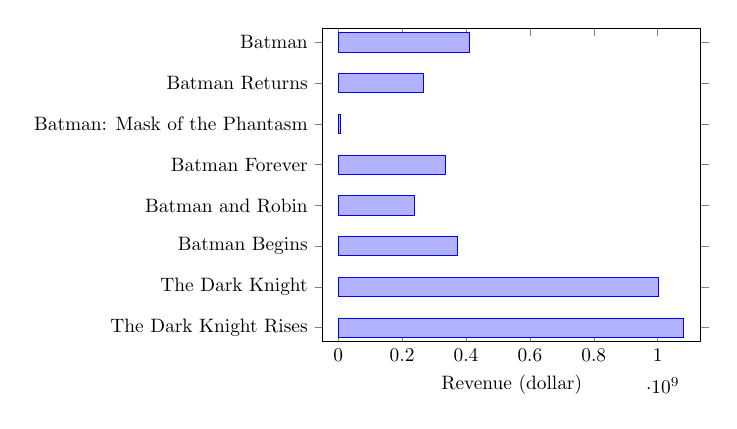
\begin{tikzpicture}[scale=.7]
  \begin{axis}[
  xbar,
  enlargelimits=0.05,
  legend style={at={(0.5,-0.2)}, anchor=north,legend columns=-1},
  ytick=data,
  symbolic y coords={The Dark Knight Rises, The Dark Knight, Batman Begins, Batman and Robin, Batman Forever, Batman: Mask of the Phantasm, Batman Returns, Batman},
  xlabel=Revenue (dollar)
  ]
  \addplot
  coordinates {
    (1080472000,The Dark Knight Rises)
    (1002000000,The Dark Knight)
    (372710000,Batman Begins)
    (238207000,Batman and Robin)
    (336529000,Batman Forever)
    (5617000,Batman: Mask of the Phantasm)
    (266822000,Batman Returns)
    (411348000,Batman)};
  \end{axis}
  \end{tikzpicture}
\end{frame}

\begin{frame}
  \frametitle{Bar Chart}
  % Source: http://mirrors.ibiblio.org/CTAN/graphics/pgf/contrib/pgfplots/doc/pgfplots.pdf
  % p.79
  \begin{center}
    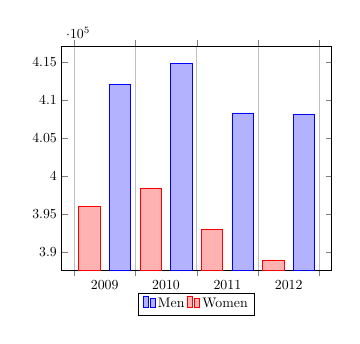
\begin{tikzpicture}[scale=.5]
    \begin{axis}[
    x tick label style={
      /pgf/number format/1000 sep=},
    xlabel=Year,
    enlargelimits=0.05,
    legend style={at={(0.5,-0.1)},
      anchor=north,legend columns=-1},
    ybar interval=0.7,
    ]
    \addplot
    coordinates {(2012,408184) (2011,408348)
      (2010,414870) (2009,412156) (2008,415 838)};
    \addplot
    coordinates {(2012,388950) (2011,393007)
      (2010,398449) (2009,395972) (2008,398866)};
    \legend{Men,Women}
    \end{axis}
    \end{tikzpicture}
  \end{center}
  Advantages
  
  \begin{itemize}
      \item Comparing categories is easier
      \item Multiple ``bars'' per category are possible
  \end{itemize}
\end{frame}


\begin{frame}
  \frametitle{Boxplot}
  \begin{columns}
    \column{.5\textwidth}
    % Source: http://mirrors.ibiblio.org/CTAN/graphics/pgf/contrib/pgfplots/doc/pgfplots.pdf
    % p.430
    \begin{tikzpicture}[scale=.9]
    \begin{axis}[x=3cm,xticklabels={},xmax=2.3]
    \addplot+[
    boxplot prepared={
      draw direction=y,
      lower whisker=5,
      lower quartile=7,
      median=8.5,
      upper quartile=9.5,
      upper whisker=10,
    },
    ]
    table[row sep=\\,y index=0] {
      data\\ 1\\ 3\\
    }
    [right,color=hgorange]
    node at
    (boxplot box cs: 1,.6)
    {outlier}
    node at
    (boxplot box cs: \boxplotvalue{lower quartile},1)
    {$Q_1$}
    node at
    (boxplot box cs: \boxplotvalue{median},1)
    {$Q_2$, median}
    node at
    (boxplot box cs: \boxplotvalue{upper quartile},1)
    {$Q_3$}
    node at
    (boxplot box cs: \boxplotvalue{upper whisker},1)
    {max}
    ;
    \end{axis}
    \end{tikzpicture}
    
    \column{.5\textwidth}
    Advantage: quick way to inspect the spread of the data and to compare several datasets.
  \end{columns}
\end{frame}

\subsection{Interpretation of Charts}

\begin{frame}
  \frametitle{Data ambiguity}    
  \framesubtitle{= not indicating what the data means.}
  
  \begin{columns}
    \column{.5\textwidth}
    \includegraphics[width=\textwidth]{les2-02}
    \column{.5\textwidth}
    Tips:
    \begin{itemize}
      \item Label the axes
      \item Add a clear title
      \item Name the unit (and, if necessary, order of magnitude)
      \item Add a label that clarifies the chart
    \end{itemize}
  \end{columns}
\end{frame}

\begin{frame}
  \frametitle{Data distortion}
  \framesubtitle{= misrepresenting data so that invalid conclusions are drawn}
  
  \bigskip
  
  \begin{center}
    \includegraphics[height=.8\textheight]{les2-03}
  \end{center}
\end{frame}

\begin{frame}
  \frametitle{Data distortion}
  
  \begin{center}
    \includegraphics[width=.8\textwidth]{les2-03-2}
  \end{center}
\end{frame}

\begin{frame}
  \frametitle{Data distraction}
  
  \begin{itemize}
    \item Avoid bells and whistles
    \item Minimize ``ink to data'' ratio
  \end{itemize}
  
  \centering
  \includegraphics[width=.3\textwidth]{les2-04}
  \includegraphics[width=.3\textwidth]{les2-05}
  
  \includegraphics[width=.3\textwidth]{les2-06}
  \includegraphics[width=.3\textwidth]{les2-07}
\end{frame}

\begin{frame}
  \frametitle{Anscombe's Quartet}
  
  \centering
  \includegraphics[height=.6\textheight]{anscombes_quartet}
  
  Four different datasets with the same statistical properties.\\ These demonstrate the importance of data visualization.
\end{frame}

\begin{frame}[plain]
  \centering
  
  \includegraphics[height=.9\textheight]{1var-datasaurus-dozen.png}
  
  ``The Datasaurus Dozen'' (Source: \url{https://www.autodeskresearch.com/publications/samestats})
\end{frame}


\end{document}